%\documentclass[journal,12pt,twocolumn]{IEEEtran}
%\usepackage{amsmath}
%\providecommand{\pr}[1]{\ensuremath{\Pr\left(#1\right)}}
%\providecommand{\cbrak}[1]{\ensuremath{\left\{#1\right\}}}
%\newcommand*{\permcomb}[4][0mu]{{{}^{#3}\mkern#1#2_{#4}}}
%\newcommand*{\comb}[1][-1mu]{\permcomb[#1]{C}}


\documentclass[journal,12pt,two column]{IEEEtran}

\usepackage[utf8]{inputenc}
\usepackage{graphicx}
\usepackage{amsmath}


%\title{Assignment 1}
%%\author{I Sai Pradeep}\\
%\date{\today}
%\textbf{Exercise 3.4, Oppenheimer}}
%\maketitle
	%\begin{abstract}
		%This document contains the solution to Oppenheimer problem 3.4(c),
	%\end{abstract}
%\begin{document}
%\maketitle
\begin{document}
	\title{\huge{Assignment 1}\\EE3900}
	\author{\Large{I Sai Pradeep}\\AI21BTECH11013}
    %\today
	\maketitle
    
	\begin{abstract}
	This document contains the solution to Oppenheimer problem 3.4(c),
	\end{abstract}
	\noindent \textbf{Question 3.4(c):}
Consider the z-transform $X(z)$ whose pole-zero plot is as shown in Figure \ref{fig:pole_zero_plt}.
\begin{figure}[!ht]
	\centering
	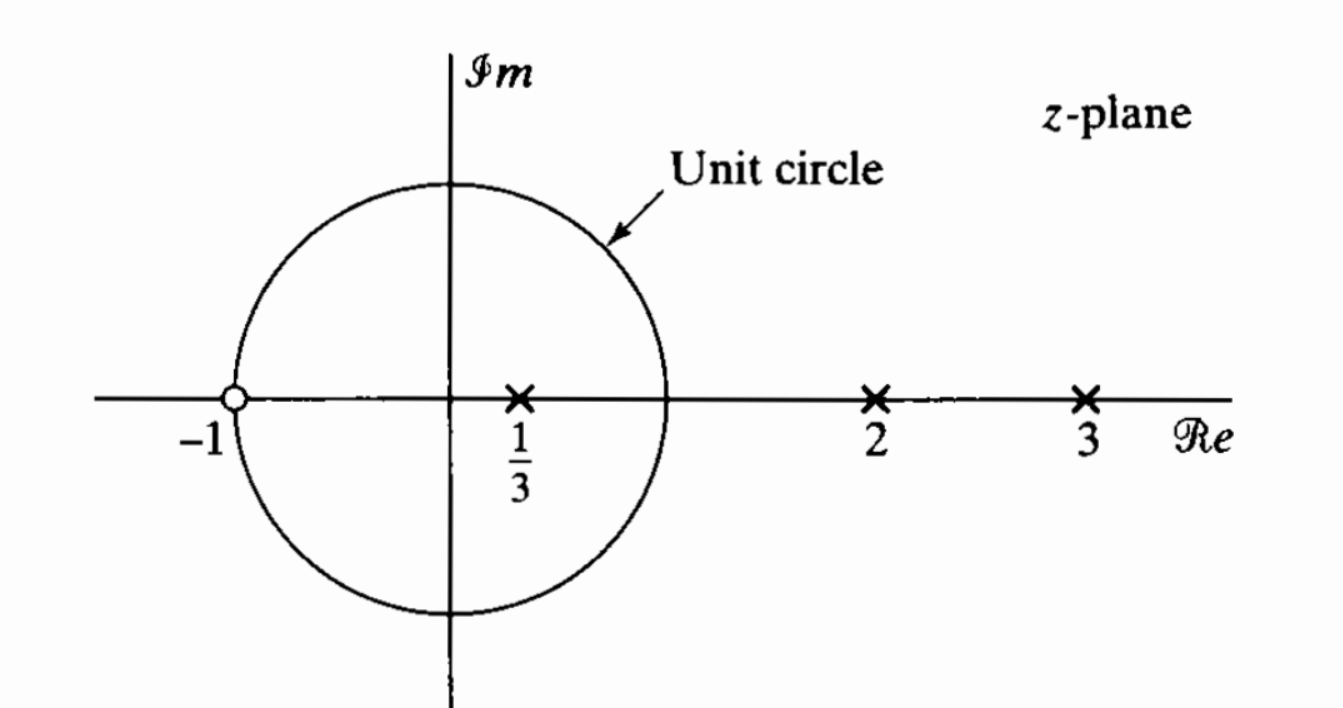
\includegraphics[width=\columnwidth]{./figs/pole_zero_plt}
	\caption{Pole Zero plot of $X(n)$}
	\label{fig:pole_zero_plt}
	\end{figure}
 \\
%Question:
Is it possible for the pole-zero plot in Figure \ref{fig:pole_zero_plt} to be associated with a sequence that is both stable and causal? If so, give the appropriate region of convergence.
	
		\textbf{Solution} For stability of the system, ROC must contain the unit circle. So, possible options is 
		\begin{align}
			|\frac{1}{3}|<|z|<|2|
		\end{align}
		For causality, the ROC must be outside of outermost pole which is 3 in this case. So, possible option is
		\begin{align}
			|z|>|3|
		\end{align}

		Since nothing is common between two, so there is no possible signal which is both stable and causal.
\end{document}
%\begin{document}
	%\title{\huge{Assignment 1}\\AI1110}
	%\author{\Large{I Sai Pradeep}\\AI21BTECH11013}
	%\maketitle
	%\begin{abstract}
	
	%\end{abstract}
	%Question
	%\noindent \textbf{Question 3.4(c):}
  %      Is it possible for the pole-zero plot in Figure \ref{P3.4-1}  to be associated with a sequence that is both stable and causal? If so, give the appropriate region of convergence. \\	
	%Solution
	%\textbf{Solution:} We have the two sequences as \frac{1}{3} < \mod{Z} < \f
	%\begin{align}
	%	P_7 &=1-(P_3+P_4+P_5+P_6) \\
	%	&= 1-(\dfrac{1}{45}+ \dfrac{1}{15} + \dfrac{1}{15} + \dfrac{1}{15}) \\
		%&= 1-\dfrac{2}{9}\\
	%	&= \dfrac{7}{9}
	%\end{align}
	%Hence, the probability that atleast one of the balls drawn from the urn is red is $\dfrac{7}{9}$.
%\end{document}